\documentclass[a4paper,12pt]{article}
\usepackage{epsfig,latexsym,amsmath,amssymb,epic,eepic,psfrag,subfigure,float,euscript,array}
\usepackage[latin1]{inputenc}
\usepackage{standalone}
\usepackage{tikz,pgf,pgfplots}

\newenvironment{exercise}[1][Uppgift]{\begin{trivlist} \item[\hskip
    \labelsep {\stepcounter{exerctr}\bfseries #1
      \arabic{exerctr}}]}{\end{trivlist}\vspace{10mm}}

\newcounter{exerctr}
\newcounter{abcctr}[exerctr]

\newcommand{\abc}{\noindent\vspace{1mm}\\ {\bf
    \stepcounter{abcctr}(\alph{abcctr})\ }}
\newcommand{\bbm}{\begin{bmatrix}}
\newcommand{\ebm}{\end{bmatrix}}
\newcommand{\point}[1]{\hfill {\bf (#1p)}\\ \vspace{-5mm}}
\newcommand{\ctrb}{\EuScript{S}}
\newcommand{\Lap}{\mathcal{L}}
\newcommand{\obsv}{\EuScript{O}}
\newcommand{\realdel}[1]{\text{Re}\left\{#1\right\}}
\newcommand{\imagdel}{\text{Im}}
\newcommand{\bC}{\mathbb{C}}
\newcommand{\bR}{\mathbb{R}}
\newcommand{\bmpv}{\begin{minipage}[t]}
\newcommand{\bmps}{\begin{minipage}[t]{45mm}}
\newcommand{\bmpm}{\begin{minipage}[t]{90mm}}
\newcommand{\bmpl}{\begin{minipage}[t]{140mm}}
\newcommand{\emp}{\end{minipage}}
\newcommand*{\zethree}{\big(z - \mexp{-3h}\big)}
\newcommand*{\mexp}[1]{\ensuremath{\mathrm{e}^{#1}}}

\newcommand*\circled[1]{\tikz[baseline=(char.base)]{
            \node[shape=circle,draw,inner sep=2pt] (char) {#1};}}

\addtolength{\topmargin}{-1cm}
\textheight 23.5cm
%\oddsidemargin 0.61cm
%\evensidemargin 0.61cm


\def\OctaveG{tf([0.5 1], [1 0 -1])}

\title{Computerized control partial exam 1 from fall semester 2016, modified}
\author{Kjartan Halvorsen}

\begin{document}

\maketitle


\begin{description}
\item[Time] September 13 17:30
\item[Place] 4101
\item[Permitted aids] The single colored page with your own notes, table of Laplace transforms, calculator
\end{description}

All answers should be readable and well motivated (if nothing else is written). Solutions/motivations should be written on the provided spaces in this exam. Use the last page if more space is needed.

\begin{center}
{\Large Good luck!} \\
\end{center}

\begin{tabular}{|l|l|}
\hline
\multicolumn{2}{|l|}{\bmpl
Matricula and name
\vspace*{18mm}
\emp}\\
\hline

\end{tabular}

\clearpage

%-----------------------------------------------------------------
\subsection*{The system}
The dynamic model of a ship with input $u$ being the rudder angle and the output $y$ being the heading (see figure \ref{fig:tanker}) can be described as a continuous-time second order system with a pole in the origin
\[ G(s) = \frac{K}{s(s + a)}. \]
For fully loaded, large tankers this dynamics is often unstable, meaning that $a<0$.  
\begin{figure}[h]
\begin{center}
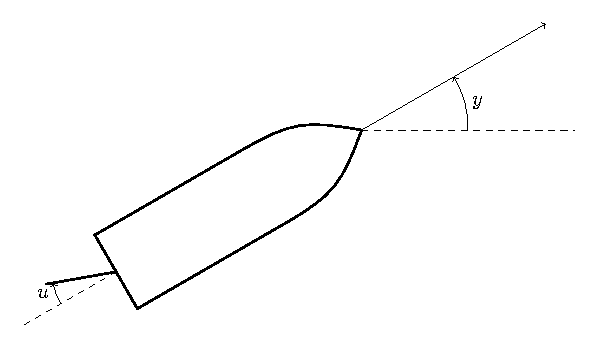
\includegraphics[width=0.8\linewidth]{tanker}
\caption{Heading of a ship controlled by rudder input.}
\label{fig:tanker}
\end{center}
\end{figure}

Consider for this exam the normalized continuous-time model of the tanker
\[ G(s) = \frac{1}{s(s - 1)}. \]

\clearpage
\subsection*{Problem 1 (50p)}

The system is sampled with sampling interval $h$ using step-invariant (zero-order hold) sampling. \textbf{Circle the correct pulse-transfer function below, and show your calculations}
\begin{enumerate}
 \item \( H(z) = \frac{(1-\mexp{h} -h)z - \big((1-h)\mexp{h}-1\big)}{(z-1)(z-\mexp{h})}\)
 \item \( H(z) = \frac{(-1+\mexp{h} -h)z - \big((1-h)\mexp{h}-1\big)}{(z-1)(z-\mexp{2h})}\)
 \item \( H(z) = \frac{(-1+\mexp{h} -h)z - \big((1-h)\mexp{h}-1\big)}{(z-1)(z-\mexp{h})}\)
 \end{enumerate}

\noindent
\fbox{
\bmpl
{\bf Derivation:}\\
\vspace*{150mm}
\emp}

\clearpage
\subsection*{Problem 2 (20p)}
Assume that the sampling period is $h=0.2$. In figure \ref{fig:complex-plane} draw the poles (crosses) and zero (circle) for both the continuous-time transfer function $G(s)$ and the  discretized pulse-transfer function $H(z)$ you determined in Problem 1.
   \begin{figure}[h]
   \begin{center}
   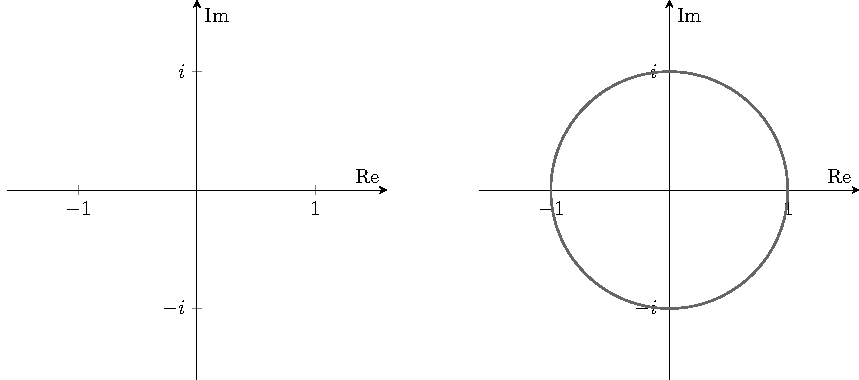
\includegraphics[]{complex-plane}
   \caption{Problem 2: Plot the poles of the continuous-time system (on the left) and the poles and zero of the discrete-time system (on the right). Indicate (with arrows and/or colors) corresponding pairs of continuous-time and discrete-time poles.}
   \label{fig:complex-plane}
   \end{center}
   \end{figure}

\noindent
\fbox{
\bmpl
{\bf Calculations:}\\
\vspace*{90mm}
\emp}

\clearpage

\subsection*{Problem 3 (40p)}
Assume, now, that the plant \(H(z) = \frac{1}{z-0.9}\) is controlled by feedback from the control error, as illustrated in figure~\ref{fig:feedback}, using the controller
\[ F(z) = K\frac{z}{z-1}. \]

\begin{figure}
\begin{center}
     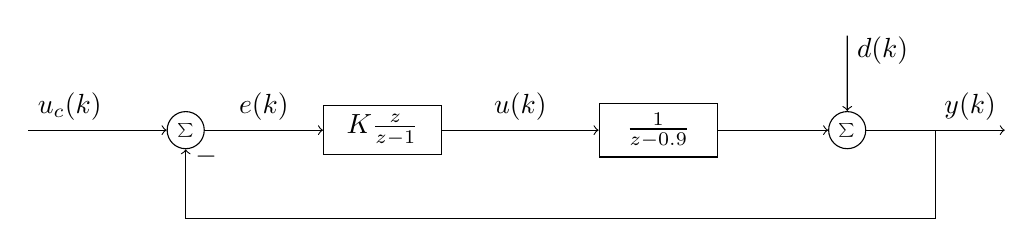
\begin{tikzpicture}[scale = 0.8, node distance=25mm, block/.style={rectangle, draw, minimum width=15mm}, sumnode/.style={circle, draw, inner sep=2pt}]
     
     \node[coordinate] (refinput) {};
     \node[sumnode, right of=refinput, node distance=20mm] (sumerr) {\tiny $\sum$};
     \node[block, right of=sumerr] (controller) {$K\frac{z}{z-1}$};
     %\node[above of=controller, node distance=6mm] {controller};
     \node[block, right of=controller, node distance=35mm] (plant) {$\frac{1}{z-0.9}$};
     \node[sumnode, right of=plant, node distance=24mm] (sum) {\tiny $\sum$};
     %\node[above of=tank, node distance=6mm] {motor};
     \node[coordinate, right of=sum, node distance=20mm] (output) {};
     \node[coordinate, above of=sum, node distance=12mm] (disturbance) {};

     \draw[->] (refinput) -- node[above, pos=0.3] {$u_c(k)$} (sumerr);
     \draw[->] (sumerr) -- node[above] {$e(k)$} (controller);
     \draw[->] (controller) -- node[above] {$u(k)$} (plant);
     \draw[->] (plant) -- (sum);
     \draw[->] (sum) -- node [coordinate] (measure)  {} node [above, near end] {$y(k)$} (output);
     \draw[->] (disturbance) -- node[right, pos=0.2] {$d(k)$} (sum);
     \draw[->] (measure) -- ++(0,-14mm) -| node[right, pos=0.95] {$-$} (sumerr);
     \end{tikzpicture}
     \caption{Feedback control from the error signal.}
     \label{fig:feedback}
   \end{center}
 \end{figure}
 
\subsubsection*{(a) 20p}

Figure~\ref{fig:rlocus} shows the root locus for the closed-loop poles with respect to the gain $K$. In figure~\ref{fig:step}, four different step plots are shown for four different values of $K$. Identify (and circle) the corresponding step plot for each value of $K$ in the table below.

\begin{center}
\begin{tabular}{cl}
\(K\) & Step plot\\\hline
0.002 & A\hspace*{2mm} B\hspace*{2mm} C\hspace*{2mm} D\\
1.0 & A\hspace*{2mm}  B\hspace*{2mm}  C\hspace*{2mm} D\\
3.0 & A\hspace*{2mm} B\hspace*{2mm}  C\hspace*{2mm} D\\
4.0 & A\hspace*{2mm} B\hspace*{2mm}  C\hspace*{2mm} D\\ \hline
\end{tabular}
\end{center}

\begin{figure}[bp]
\begin{center}
\begin{tikzpicture}
    \node[anchor=south west,inner sep=0] at (0,0) {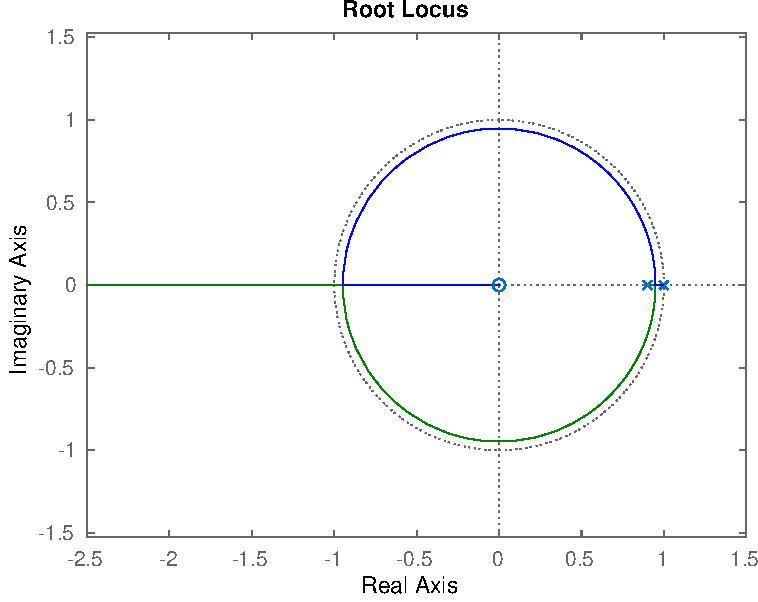
\includegraphics[width=0.5\linewidth]{p2_rlocus_rlocus-crop}};
    \node[coordinate, pin={[pin distance=20mm] 80:{$K=0.003$}}] at (7.17,3.47) {};
    \node[coordinate, pin={[pin distance=20mm] 115:{$K=3.8$}}] at (3.77,3.47) {};
\end{tikzpicture} 

\caption{Root locus wrt the gain $K$.}
\label{fig:rlocus}
\end{center}
\end{figure}

\begin{figure}[tp]
\begin{center}
\begin{tabular}{cc}
A & B\\
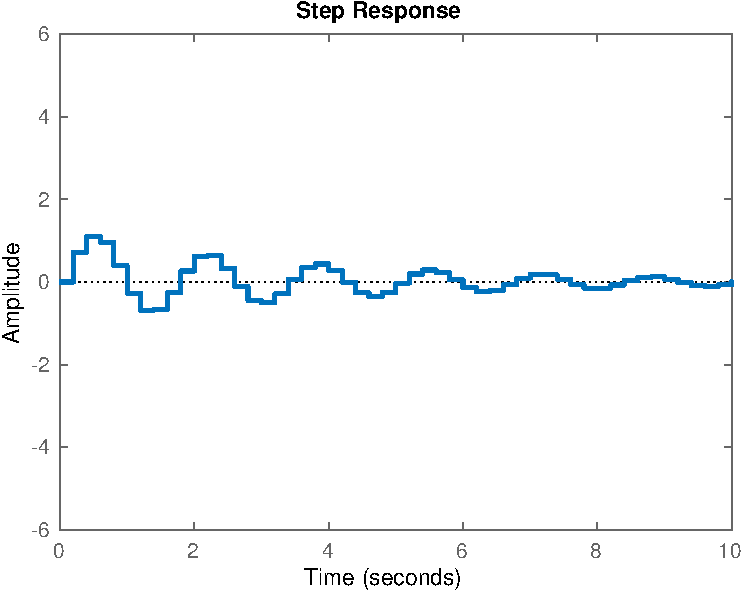
\includegraphics[width=0.4\linewidth]{step-plot-3-crop}
&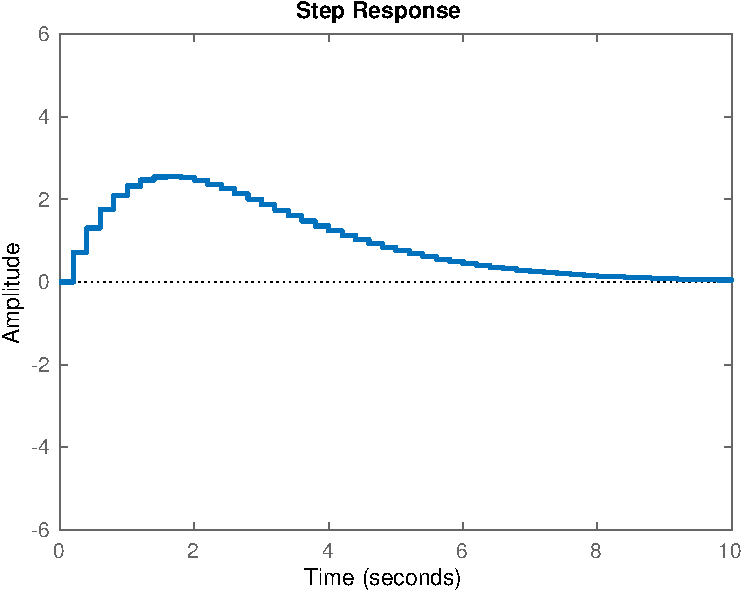
\includegraphics[width=0.4\linewidth]{step-plot-1-crop}\\
C & D\\
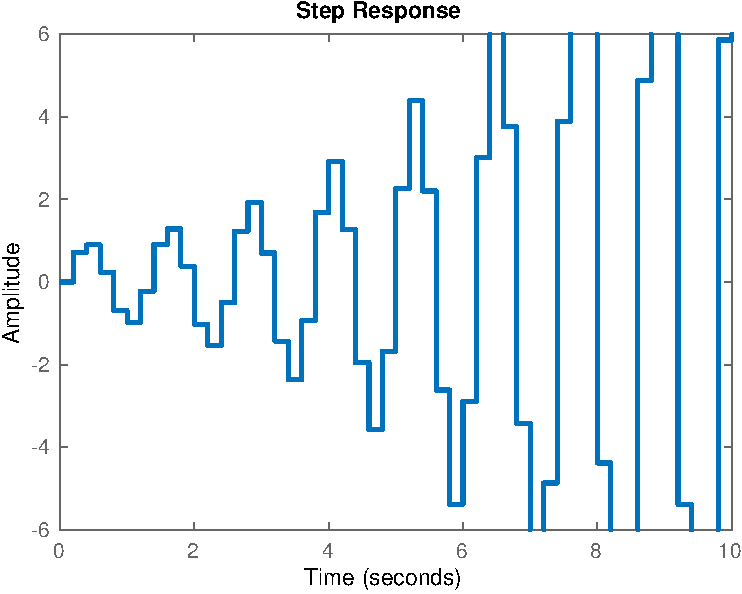
\includegraphics[width=0.4\linewidth]{step-plot-5-crop}
&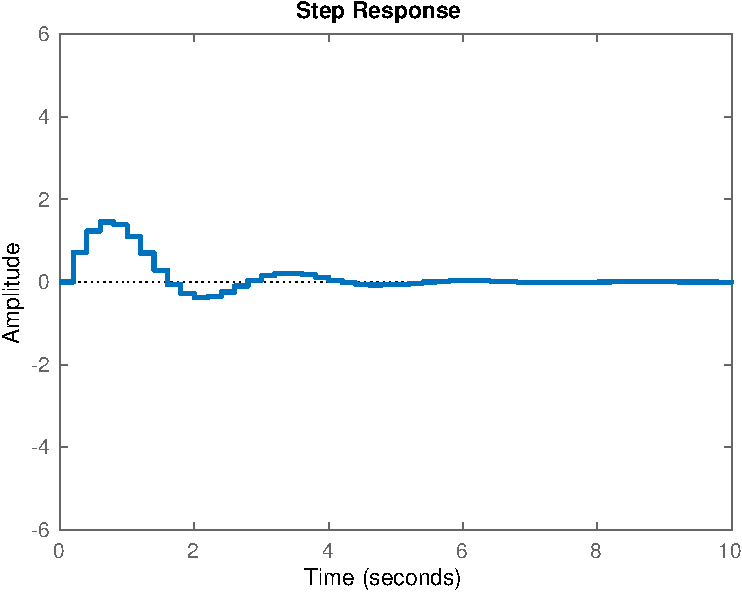
\includegraphics[width=0.4\linewidth]{step-plot-2-crop}

\end{tabular}
\caption{Step responses for different values of $K$.}
\label{fig:step}
\end{center}
\end{figure}

\clearpage
\subsubsection*{(b) 20p}

Determine the gain $K$ so that the closed loop system has poles with realpart equal to $0.7$.


\noindent
\fbox{
\bmpl
{\bf Solution:}\\
\vspace*{150mm}
\emp}

\cleardoublepage

\noindent
{\bf If necessary,} you can continue your solutions on this page. Mark clearly which problem the solution corresponds to.


%\end{document}

%*****************************************************************
%*****************************************************************
\newpage
\setcounter{page}{1}

\section*{Solutions}
\subsection*{Problem 1}
   First calculate the step-response of the continous-time system
   \[Y(s) = G(s)\frac{1}{s} = \frac{1}{s^2(s-1)} = \frac{1}{s-1} - \frac{1}{s} - \frac{1}{s^2}.\]
   The inverse Laplace-transform gives
   \[ y(t) = \mexp{t} - 1 - t\]
   Sampling this function gives
   \[ y(kh) = \mexp{kh} -1 - kh\]
   which has the Z-transform
   \[Y(z) = \frac{z}{z - \mexp{h}} - \frac{z}{z-1} - \frac{hz}{(z-1)^2}\]
   Dividing the z-transform of the system response to that of the input (the step) gives
   \begin{align*}
   H(z) &= \frac{Y(z)}{U(z)} = \frac{z-1}{z}Y(z) = \frac{z-1}{z-\mexp{h}} - 1 - \frac{h}{z-1}\\
        &= \frac{(z-1)^2 - (z-1)(z-\mexp{h}) - h(z-\mexp{h})}{(z-1)(z-\mexp{h})}\\
	&= \frac{(z-1)(z-1 -z + \mexp{h}) - hz + h\mexp{h}}{(z-1)(z-\mexp{h})}\\
        &= \frac{ (\mexp{h} - 1 -h)z - (\mexp{h}-1-h\mexp{h})}{(z-1)(z-\mexp{h})}\\
        &= \frac{ (\mexp{h} - 1 -h)z - \big( (1-h)\mexp{h}-1\big)}{(z-1)(z-\mexp{h})}\\
   \end{align*}

   The correct pulse transfer function is the third.

\subsection*{Problem 2}
The discrete-time poles are in $z=1$ and $z=\mexp{0.2} \approx 1.22$. The zero is  in 
\[ z = - \frac{(1-h)\mexp{0.2} - 1}{\mexp{0.2} - 1 -h} \approx -1.07. \]
\begin{center}
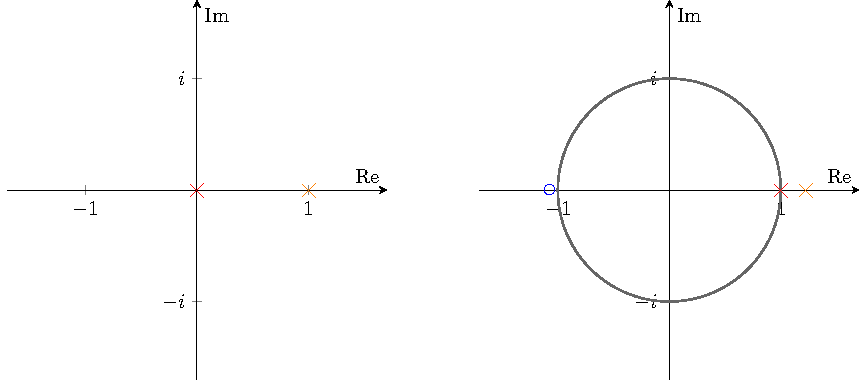
\includegraphics[width=0.8\linewidth]{complex-plane-facit}
\end{center}
 
\subsection*{Problem 3}

\subsubsection*{(a)}

The root locus starts with two poles at $1$ and $0.9$. For small values of $K$ we will have poles that are slow and completely damped. The only such response is \textbf{B}. As $K$ increases we will have closed-loop poles that follows the unit circle a bit inside it. The poles will have little damping and will increase in speed with $K$. Finally, one pole move outside the unit circle, and the system becomes unstable. It is easy to see the response that is slow (B) and unstable (C). It is a bit difficult to read off the difference in osciallation period between the other two responses. In summary, we get

\begin{center}
\begin{tabular}{cl}
\(K\) & Step plot\\\hline
0.002 & A\hspace*{2mm} \circled{B}\hspace*{2mm} C\hspace*{2mm} D\\
1.0 & A\hspace*{2mm}  B\hspace*{2mm}  C\hspace*{2mm} \circled{D}\\
3.0 & \circled{A}\hspace*{2mm} B\hspace*{2mm}  C\hspace*{2mm} D\\
4.0 & A\hspace*{2mm} B\hspace*{2mm}  \circled{C}\hspace*{2mm} D\\ \hline
\end{tabular}
\end{center}

\subsubsection*{(b)}

The closed-loop system from command signal to the output is
\[ H_c(z) = \frac{K \frac{z}{z-1}\frac{1}{z-0.9}}{1 + K \frac{z}{z-1}\frac{1}{z-0.9}} = \frac{Kz}{(z-1)(z-0.9) + Kz}. \]
The characteristic equation is 
\[ (z-1)(z-0.9) + Kz = z^2 - (1.9-K)z + 0.9 = 0 \]
with solution
\[ z = \frac{1.9-K}{2} \pm \frac{1}{2}\sqrt{(1.9-K)^2 - 5.6}. \]
We know from the root locus that for a value of  $K$ that gives poles with real part $0.7$, then the poles are complex-conjugated and so the expression under the root sign must be negative. The real part is given by the first term in the solution to the quadratic equation. We get
\[ \frac{1.9-K}{2} = 0.7 \quad \Rightarrow \quad K = 1.9-1.4 = 0.5 \]

\end{document}
